\documentclass[a4paper,10pt]{report}
\usepackage[utf8]{inputenc}
\usepackage{amsmath,amsfonts,amssymb}
\usepackage[margin=2cm]{geometry}
\usepackage{indentfirst}
\usepackage{subcaption,graphicx,float}
\usepackage{todonotes}

% Title Page
\title{Interpolation} %TODO: Come up with a better title
\author{Milos Micik}


\begin{document}
\maketitle

\begin{abstract}
\todo{Add abstract}
\end{abstract}

\chapter{Introduction}
\todo{Add introduction.}

\chapter{Interpolation in 1D}
In one dimensional interpolation we have decided to compare interpolation methods using Bezier curves and cubic polynomial splines. Both methods use piecewise polynomials to trace a curve defined by knot points and information about the first derivatives.

\todo{Possibly add a bit of theory to splines.}

In 1D, the interpolation task is nearly straightforward. The only issue that can arise is when the data to be interpolated is discretized. This could occur for example when collecting data from a measurement where the measuring device has a finite precision and can only detect change in the observed quantity in steps.
\begin{figure}[h]
 \centering
 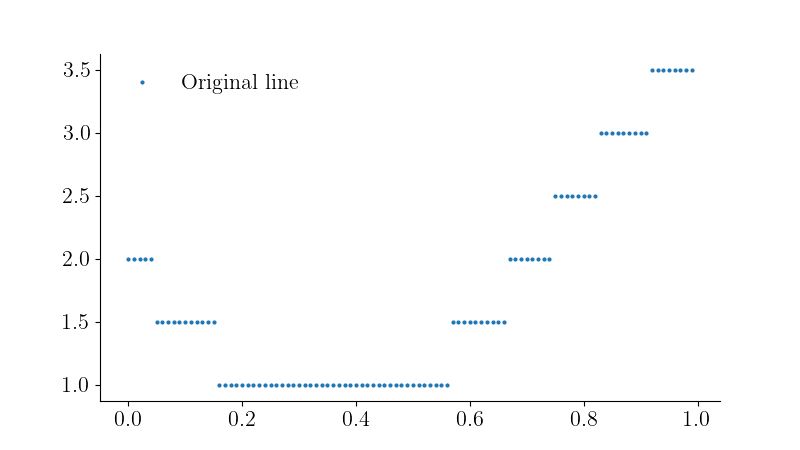
\includegraphics[width=.6\textwidth]{../images/1D_Function.png}
 % 1D_Function.png: 800x450 px, 100dpi, 20.32x11.43 cm, bb=0 0 576 324
 \caption{An example of discretized 1D data.}
 \label{fig:1D_fun}
\end{figure}

If we were to run the interpolation on such data without any adjustments, the polynomials would try to fit every single point in the collinear segments, producing a curve not too different from what we started with. Therefore in this case pre-processing of the data is required.

The pre-processing we have chosen assumes that the discretized data is obtained by rounding the real-data observation. For example, in Figure \ref{fig:1D_fun}, the collinear segment from $x\approx0.15$ to $x\approx0.55$ is represented in the data with $y$ value $1.0$, however by our assumption we know that the real values could have been anywhere in the interval $[0.75, 1.25)$. The pre-processing algorithm simply isolates a midpoint from a collinear region of points. Where the collinear region is a local maximum or minimum, we isolate two point instead, $1/3$ and $2/3$ along the collinear segment.

Using this algorithm, we can now interpolate any discretized curves in 1D. An example of it working in action can be seen in Figure \ref{fig:1D_fun_interpolated}:
\begin{figure}[H]
    \centering
    \begin{subfigure}{0.6\textwidth}
        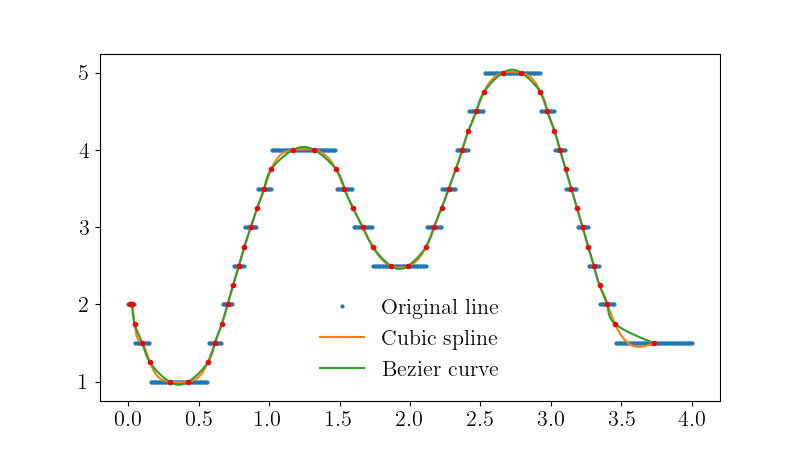
\includegraphics[width=\textwidth]{../images/1D_Function_Interpolated.png}
        % 1D_Function_Interpolated.png: 800x450 px, 100dpi, 20.32x11.43 cm, bb=0 0 576 324
    \end{subfigure}
    \hfill
    \begin{subfigure}{0.39\textwidth}
        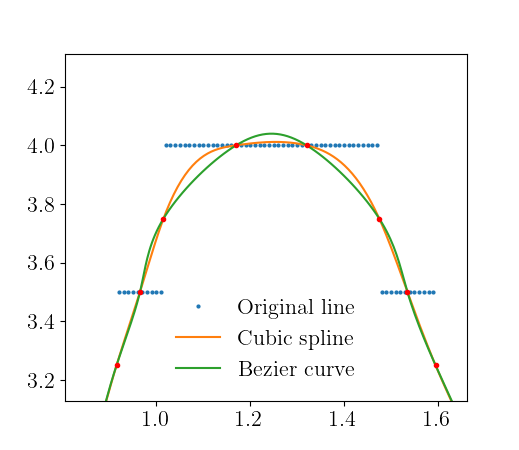
\includegraphics[width=\textwidth]{../images/1D_Function_Interpolated_Zoomed.png}
        % 1D_Function_Interpolated_Zoomed.png: 800x450 px, 100dpi, 20.32x11.43 cm, bb=0 0 576 324
    \end{subfigure}
    \caption{An example of curves interpolated from discretized 1D data.}
    \label{fig:1D_fun_interpolated}
\end{figure}

Note the subtle difference between the Bezier curve and the cubic spline. In segments which are relatively straight, their shape is very similar. However, the difference at places where the curve takes sharper turn is more noticeable. The cubic spline seems to achieve much better results, introducing less irregularities and copying the original data curve more smoothly. This does not come as a surprise, as cubic splines are expected to have \textit{$C^2$} continuity, whereas Bezier curves are only \textit{$C^1$} continuous.

\chapter{Interpolation in 2D}
\section{Parametric Curves}\label{sec:param_curve}
Interpolating parametric curves in 2D (technically in any dimension) is very similar to interpolating in 1D. It might require different functions when implementing these in a programming language, but the algorithm is the same - if the data is discretized, we need to first isolate points from collinear segments.
\begin{figure}[H]
    \centering
    \begin{subfigure}{0.49\textwidth}
        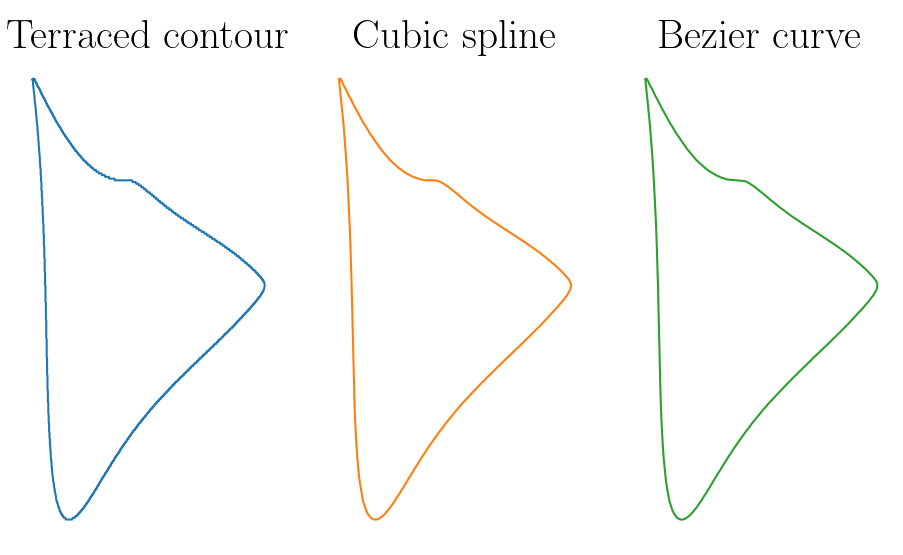
\includegraphics[width=\textwidth]{../images/2D_Contour.png}
    \end{subfigure}
    \hfill
    \begin{subfigure}{0.49\textwidth}
        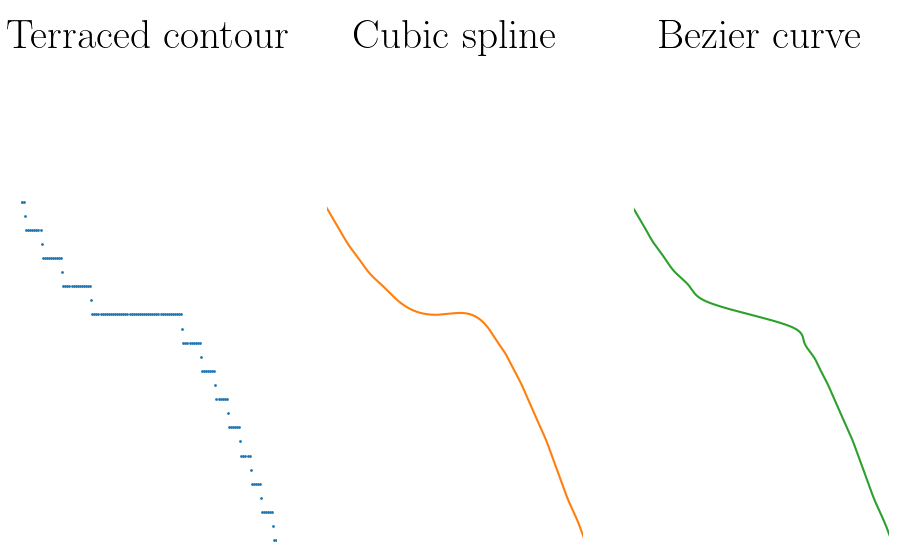
\includegraphics[width=\textwidth]{../images/2D_Contour_Zoomed.png}
    \end{subfigure}
    \caption{An example of parametric curves interpolated from discretized parametric 1D curve in 2D.}
    \label{fig:2D_parametric_curve}
\end{figure}

The same observation about the continuity holds in this case - cubic splines produce curves which look more natural.

\section{Countour Lines of a Bivariate Function}
There are many reasons why we might want to interpolate contours of a bivariate function. Computer simulations or numerical analysis methods work with discretized or rasterized input dimensions and the contours resulting from them might not be in the required resolution. Rather than having the simulation to run in a higher resolution, we may instead choose to interpolate the results, which is in most cases cheaper computationally.

Interpolating contour lines of bivariate functions mapping a 2D space to a scalar can be done by representing the contours as parametric curves. As an example, we will use digital elevation maps (DEMs) of regions from Scotland.

Isolating the contours in the first place can be done by regular marching square algorithm. The algorithm usually returns the contours already parametrized by an arbitrary parameter, therefore we can interpolate them the same way as we interpolated parametric curves in Section \ref{sec:param_curve}.

\begin{figure}[H]
    \centering
    \begin{subfigure}{\textwidth}
        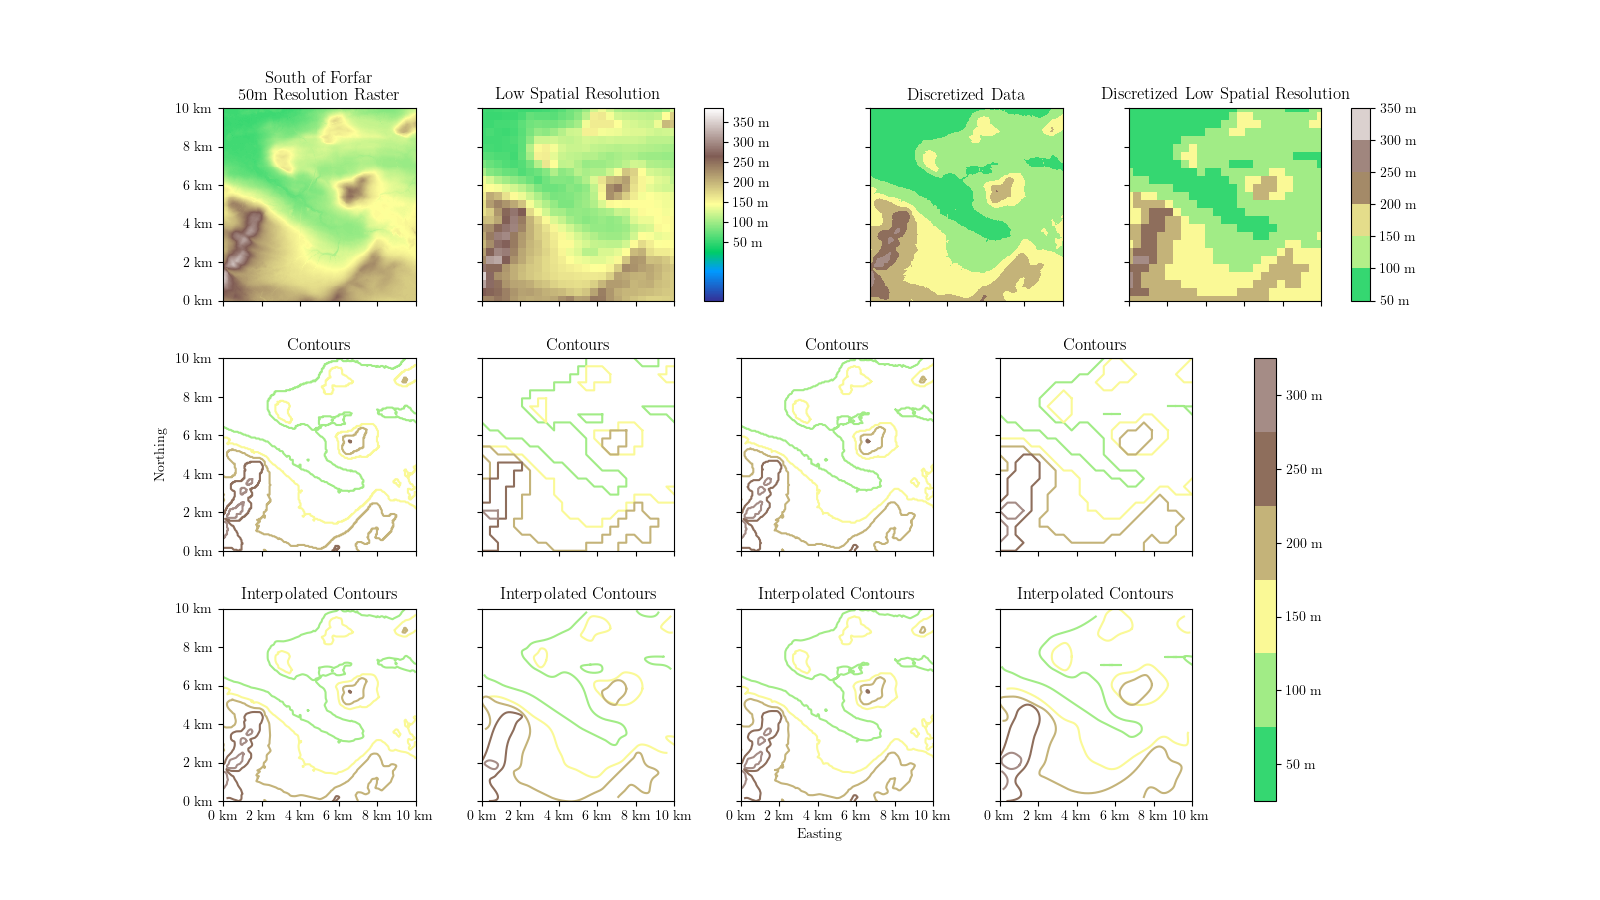
\includegraphics[width=1\textwidth]{../images/NO44/2D_Contour_Interpolation.png}
        % 2D_Contour_Interpolation.png: 1600x900 px, 100dpi, 40.64x22.86 cm, bb=0 0 1152 648
    \caption{Elevation data from near Forfar (UK ordnance tile NO44)}
    \end{subfigure}
    \begin{subfigure}{\textwidth}
        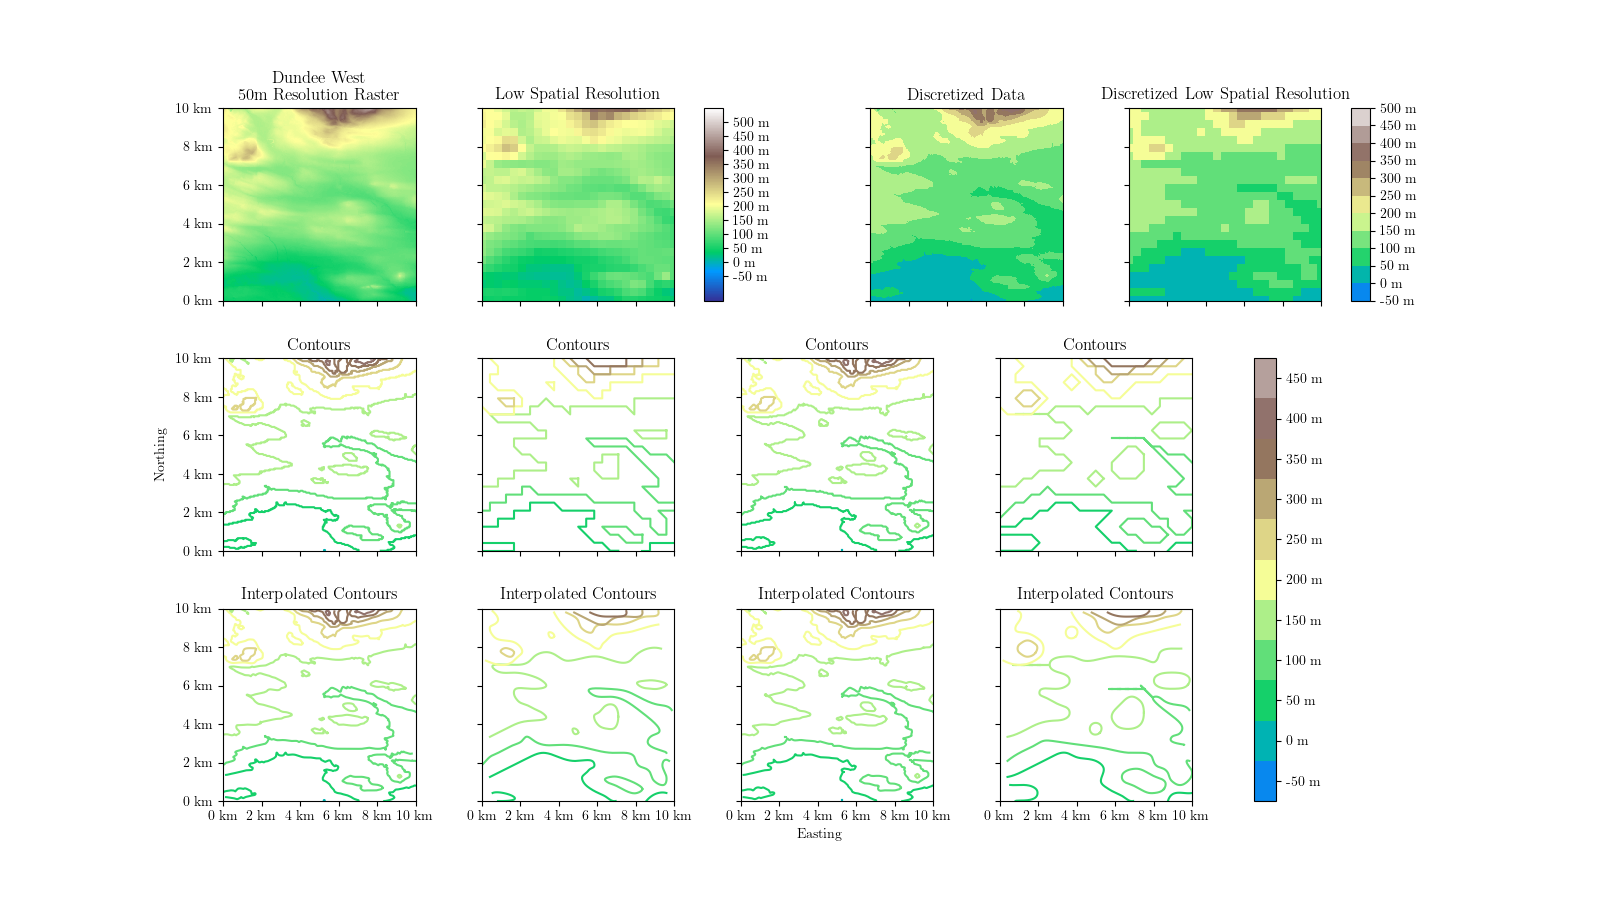
\includegraphics[width=1\textwidth]{../images/NO33/2D_Contour_Interpolation.png}
        % 2D_Contour_Interpolation.png: 1600x900 px, 100dpi, 40.64x22.86 cm, bb=0 0 1152 648
    \caption{Elevation data from west Dundee (UK ordnance tile NO33)}
    \end{subfigure}
    \caption{CInterpolation of elevation contours from data with various resolution.}
    \label{fig:2D_contour}
\end{figure}

We can see on Figure \ref{fig:2D_contour} that this approach does work quite nicely for cases when the spatial resolution is low. The contour levels can be chosen arbitraily and we should always be left with smooth contours. However, the drawbacks of this approach are that in case of discretized data, we are unable to produce contours of any level other than those of the data. For this, we would need to interpolate the data itself, as is discussed in the next section.

\section{Bivariate Function}
There are two main different cases when interpolating bivariate functions. One is that the spatial resolution of the 2D space is lower than required. In this case, the 2D space is sampled sparsely and the goal is to interpolate the function to a denser grid. The other reason is that the image of the function is discretized. The surface and it's derivatives are discontinuous, and producing a colormesh or a 3D visualisation of such data produces terraced surface. Hence we may wish to interpolate these terraces to produce a smooth surface.

\todo{Insert figure of low res data and discretized data}

In the case where the domain is sampled sparsely, but is still on a regular grid, using bivariate spline interpolation is one of the fastest and most reliable methods to interpolate the data. We've used bicubic interpolation when interpolating DEMs in our examples, but in other cases using other degrees of polynomials is also valid and the choice should perhaps be motivated by the problem.

Analogously to 1D, interpolating a discretized image of a function requires us to pre-process the data and isolate some subset of points. This is perhaps a step which depends on the nature of the data that we are trying to interpolate.

In the case of our  DEM examples, we assume that in a discretized DEM, a particular value represents real height which is equal or higher than the value. In other words, the discretized values were created by rounding down to the nearest level. Therefore, the only real values truly preserved by the discretized data representation is located on the curves where two coplanar regions meet - on the contour lines. The elevation level of the contour is then determined by the higher value of the two coplanar regions.

By isolating contours from the discretized data we obtain a set of irregularly spaced points in the domain. Using bicubic interpolation therefore is not a valid option. There are two alternative method we investigate in this report. One uses Delaunay triangulation to produce a triangular mesh from the isolated points, and then uses either barycentric interpolation or Clough-Tocher scheme (which in turn uses piecewise cubic interpolating Bezier polynomials). Other option is to use Radial basis function (RBF) interpolation.

\todo{Possibly include theory to RBF, Delaunay and Clough-Tocher?}

\begin{figure}[H]
    \centering
    \begin{subfigure}{\textwidth}
        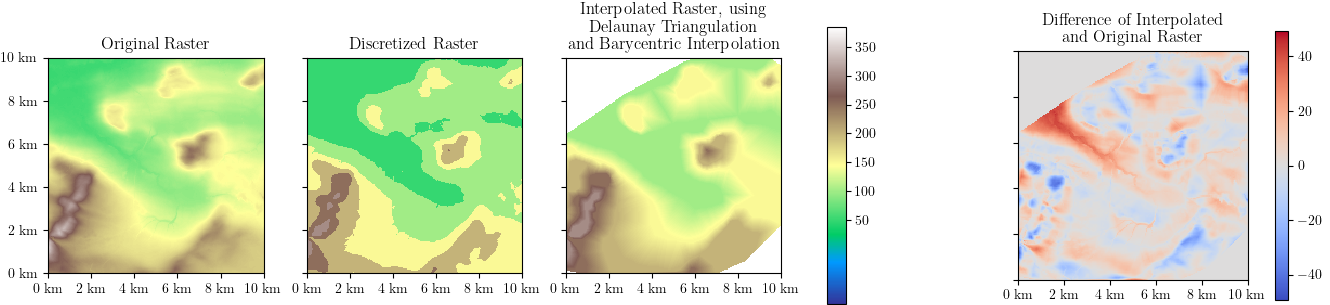
\includegraphics[width=1\textwidth]{../images/differences/Delaunay_Triangulation_and_Barycentric_Interpolation_2D.png}
        % 2D_Contour_Interpolation.png: 1600x900 px, 100dpi, 40.64x22.86 cm, bb=0 0 1152 648
    \caption{Delaunay triangulation used together with barycentric interpolation.}
    \end{subfigure}
    \begin{subfigure}{\textwidth}
        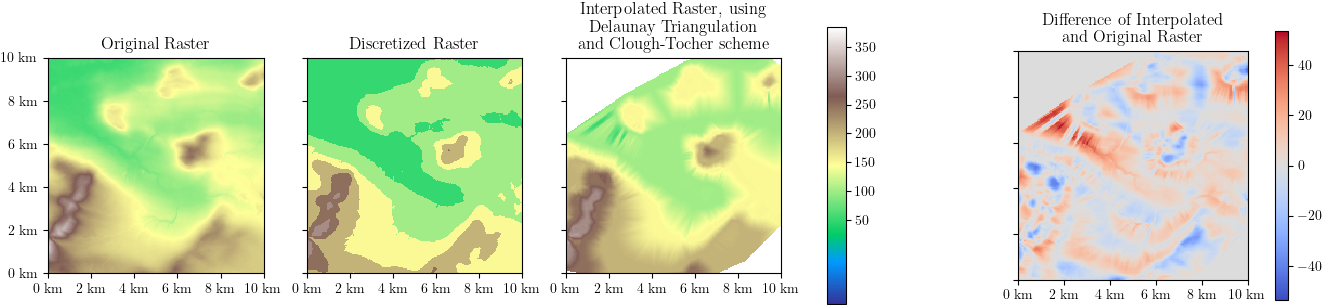
\includegraphics[width=1\textwidth]{../images/differences/Delaunay_Triangulation_and_Clough-Tocher_scheme_2D.png}
        % 2D_Contour_Interpolation.png: 1600x900 px, 100dpi, 40.64x22.86 cm, bb=0 0 1152 648
    \caption{Delaunay triangulation used together with Clough-Tocher scheme.}
    \end{subfigure}
    \begin{subfigure}{\textwidth}
        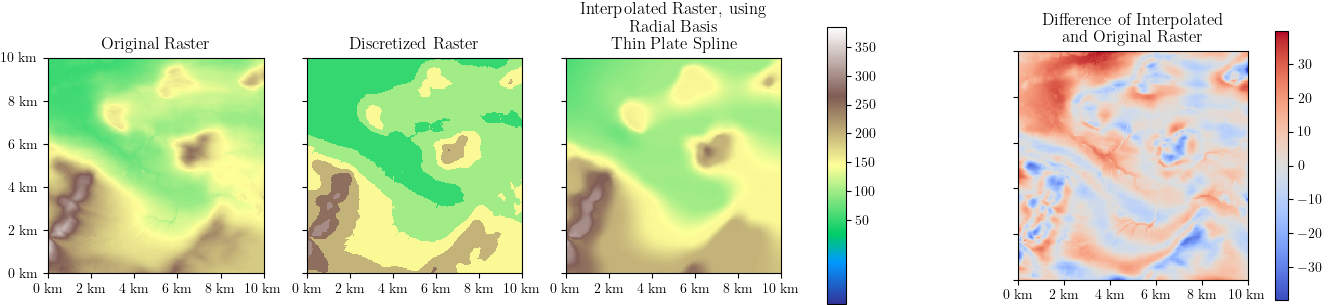
\includegraphics[width=1\textwidth]{../images/differences/Radial_Basis_Thin_Plate_Spline_2D.png}
        % 2D_Contour_Interpolation.png: 1600x900 px, 100dpi, 40.64x22.86 cm, bb=0 0 1152 648
    \caption{Radial basis function interpolation using thin plate spline radial function.}
    \end{subfigure}
    \caption{Comparison of various interpolation methods using elevation data from UK ordnance tile NO44 (South of Forfar).}
    \label{fig:2D_discretized_comparison}
\end{figure}

\begin{figure}[H]
    \centering
    \begin{subfigure}{.32\textwidth}
        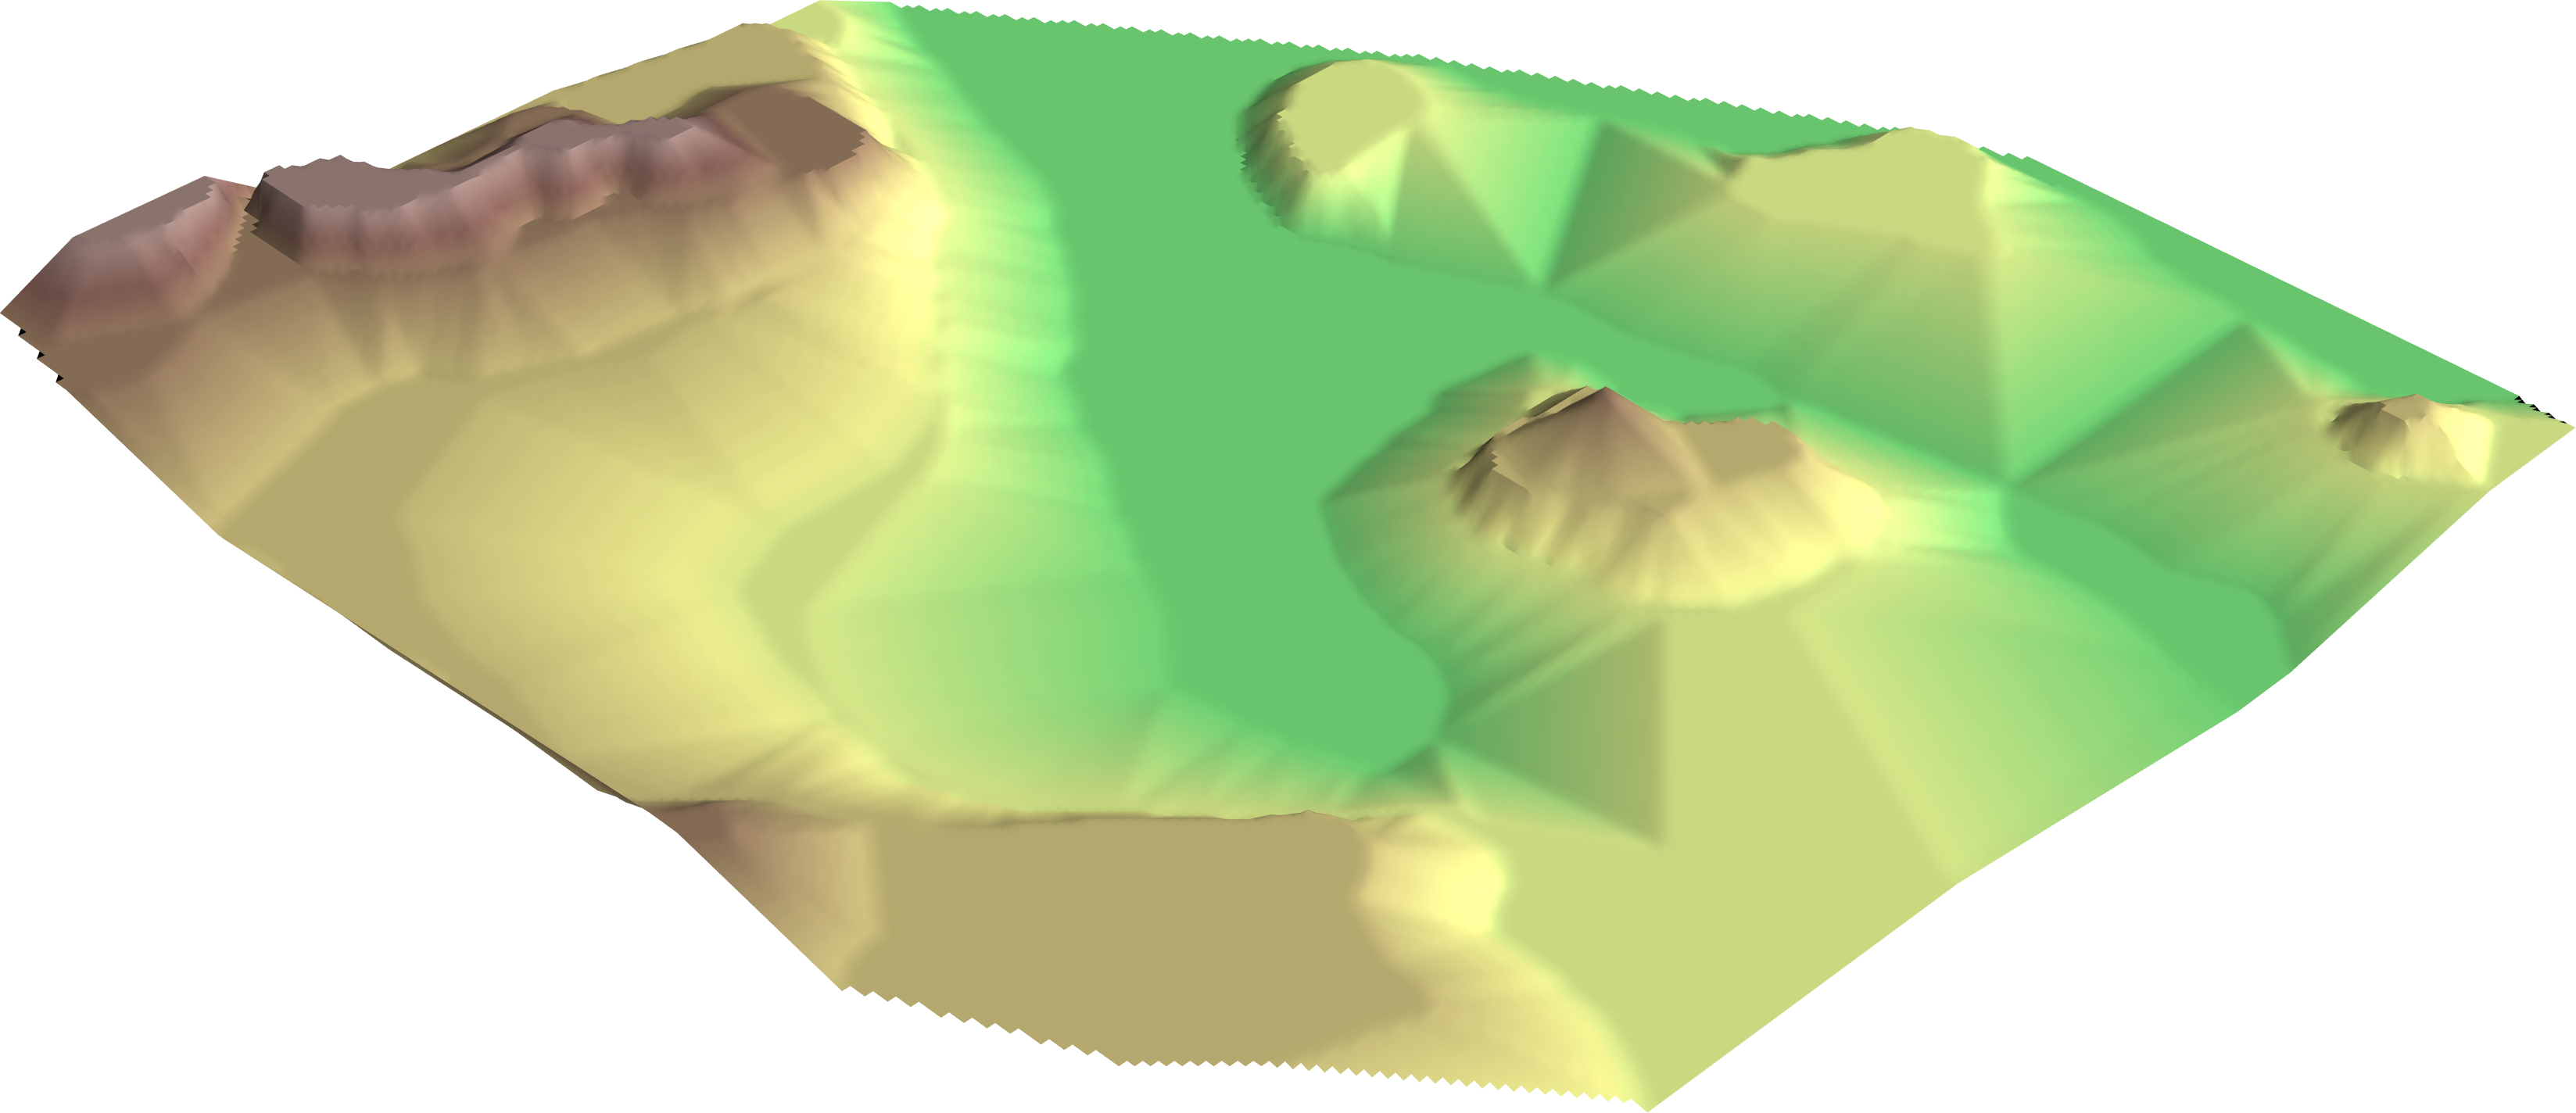
\includegraphics[width=\textwidth]{../images/differences/Delaunay_Triangulation_and_Barycentric_Interpolation_3D.png}
        % 2D_Contour_Interpolation.png: 1600x900 px, 100dpi, 40.64x22.86 cm, bb=0 0 1152 648
    \caption{Delaunay triangulation used together with barycentric interpolation.}
    \end{subfigure}
    \hfill
    \begin{subfigure}{.32\textwidth}
        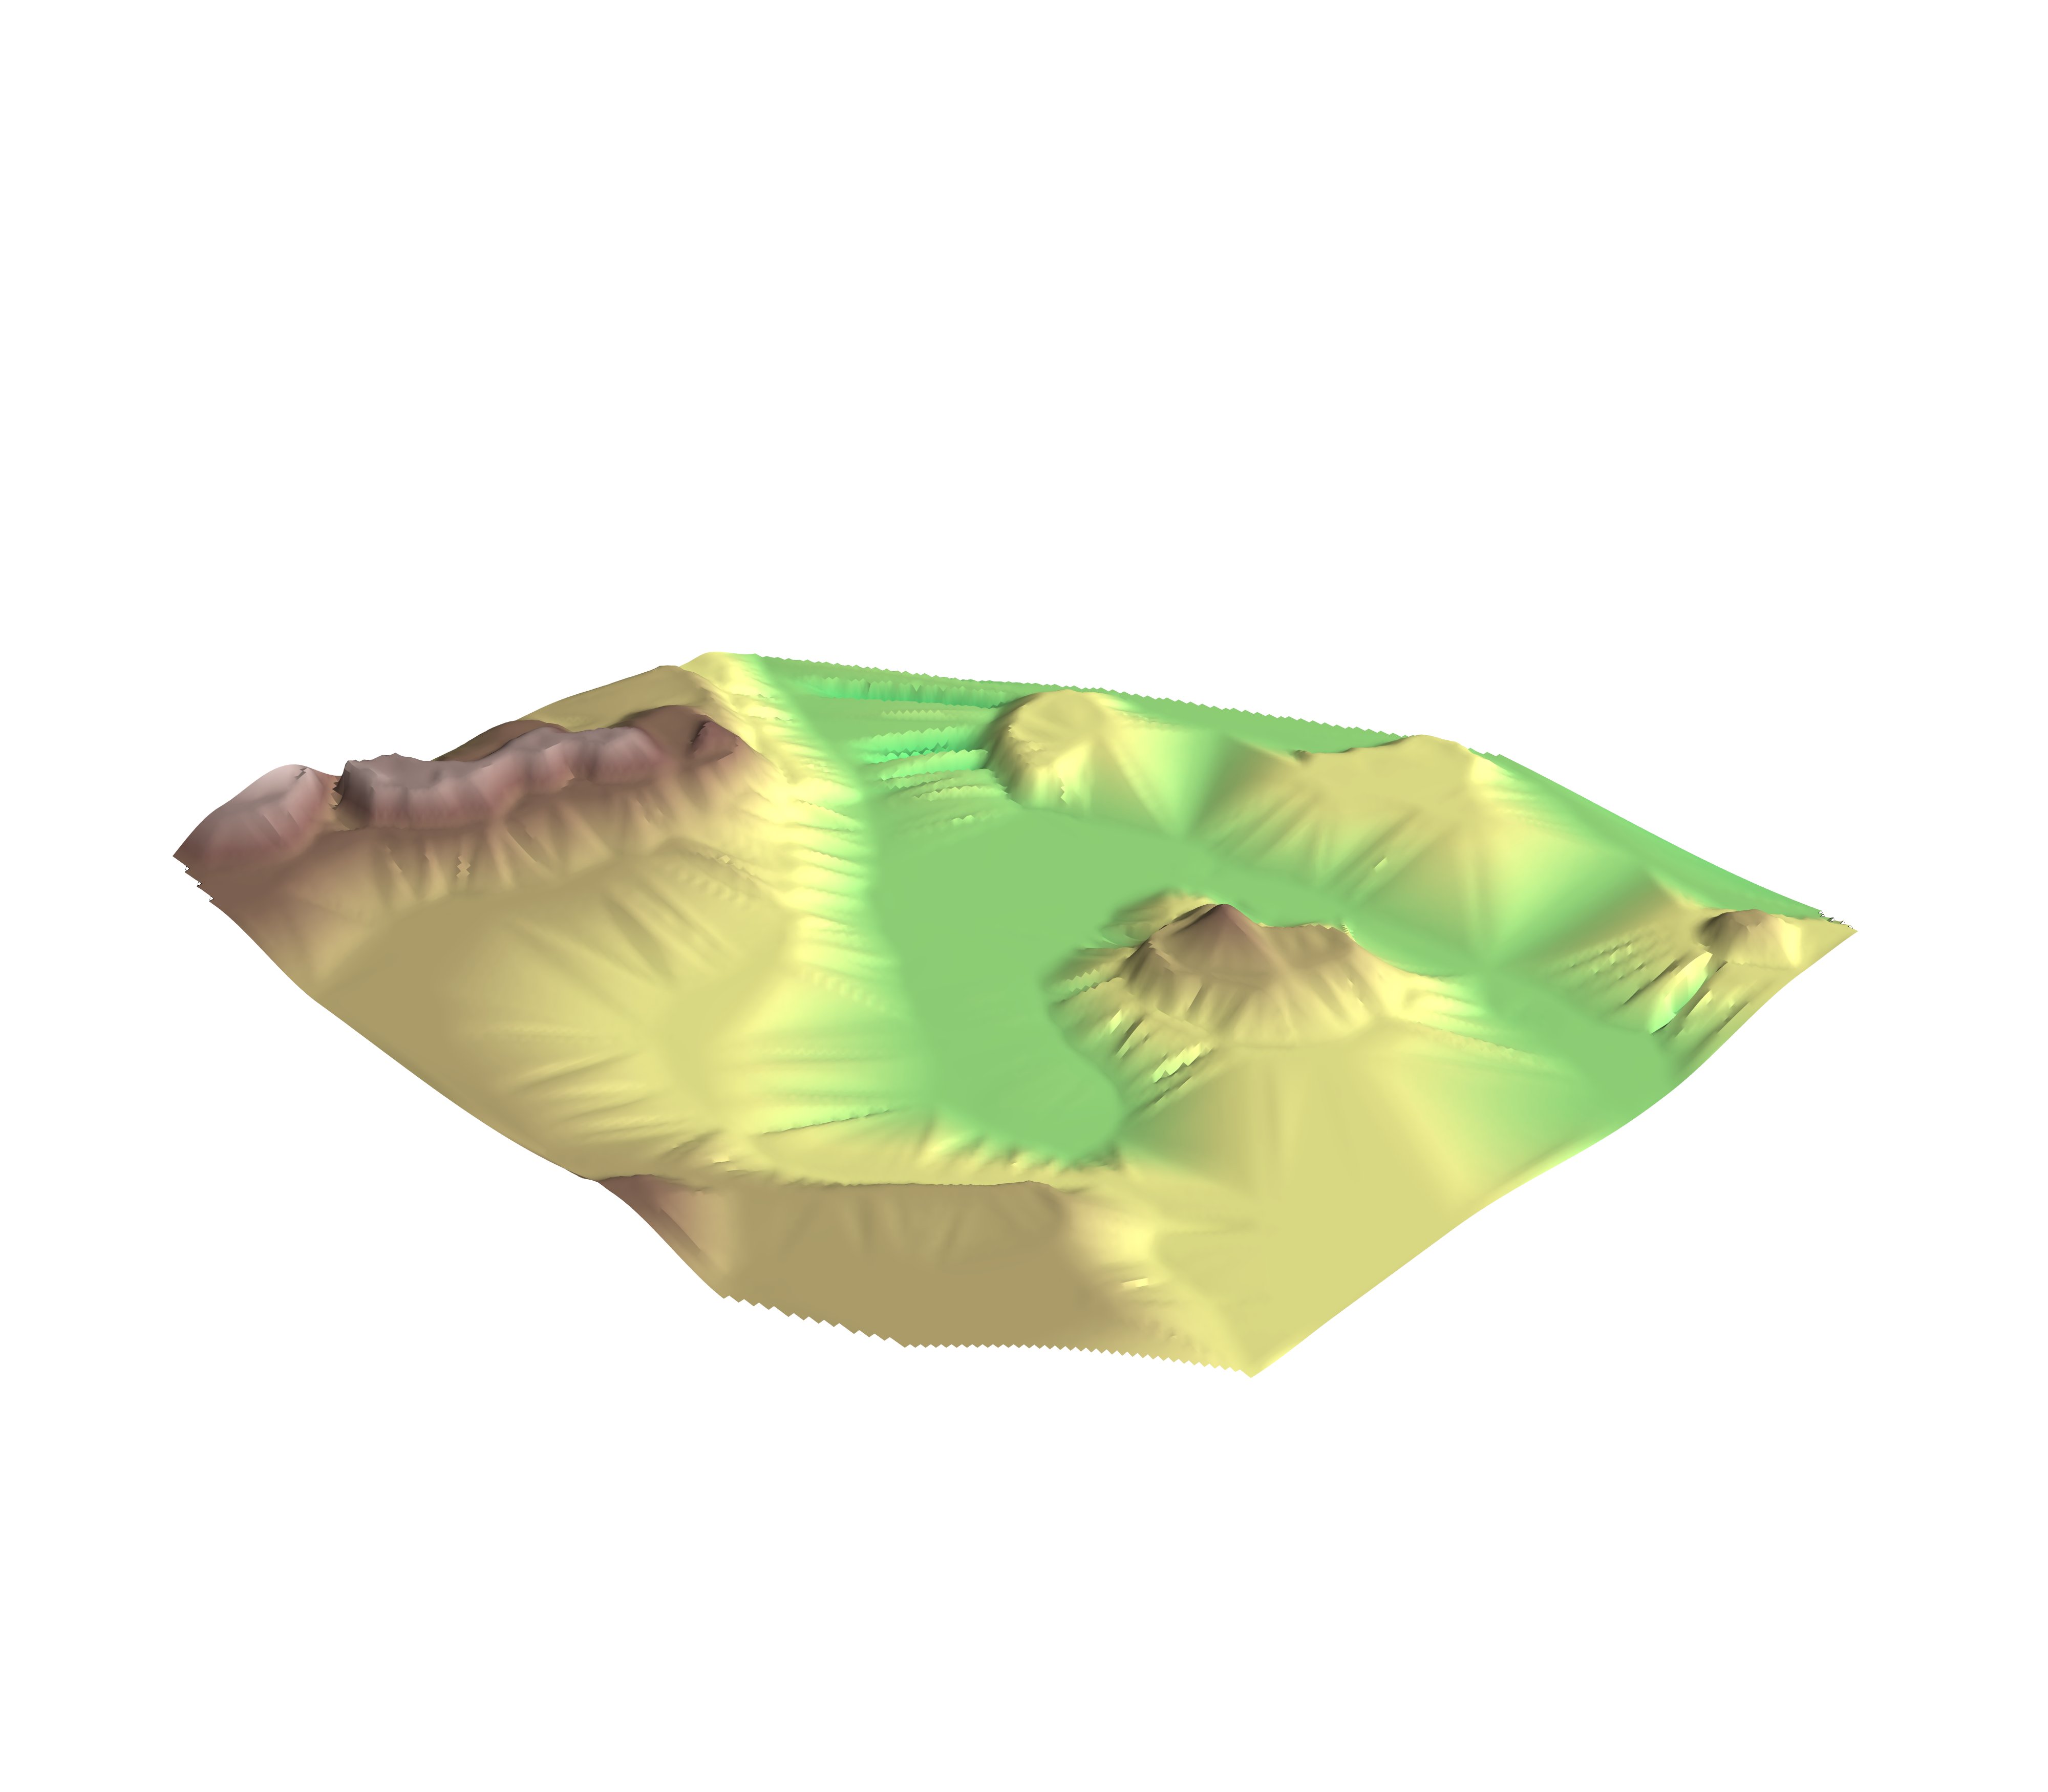
\includegraphics[width=\textwidth]{../images/differences/Delaunay_Triangulation_and_Clough-Tocher_scheme_3D.png}
        % 2D_Contour_Interpolation.png: 1600x900 px, 100dpi, 40.64x22.86 cm, bb=0 0 1152 648
    \caption{Delaunay triangulation used together with Clough-Tocher scheme.}
    \end{subfigure}
    \hfill
    \begin{subfigure}{.32\textwidth}
        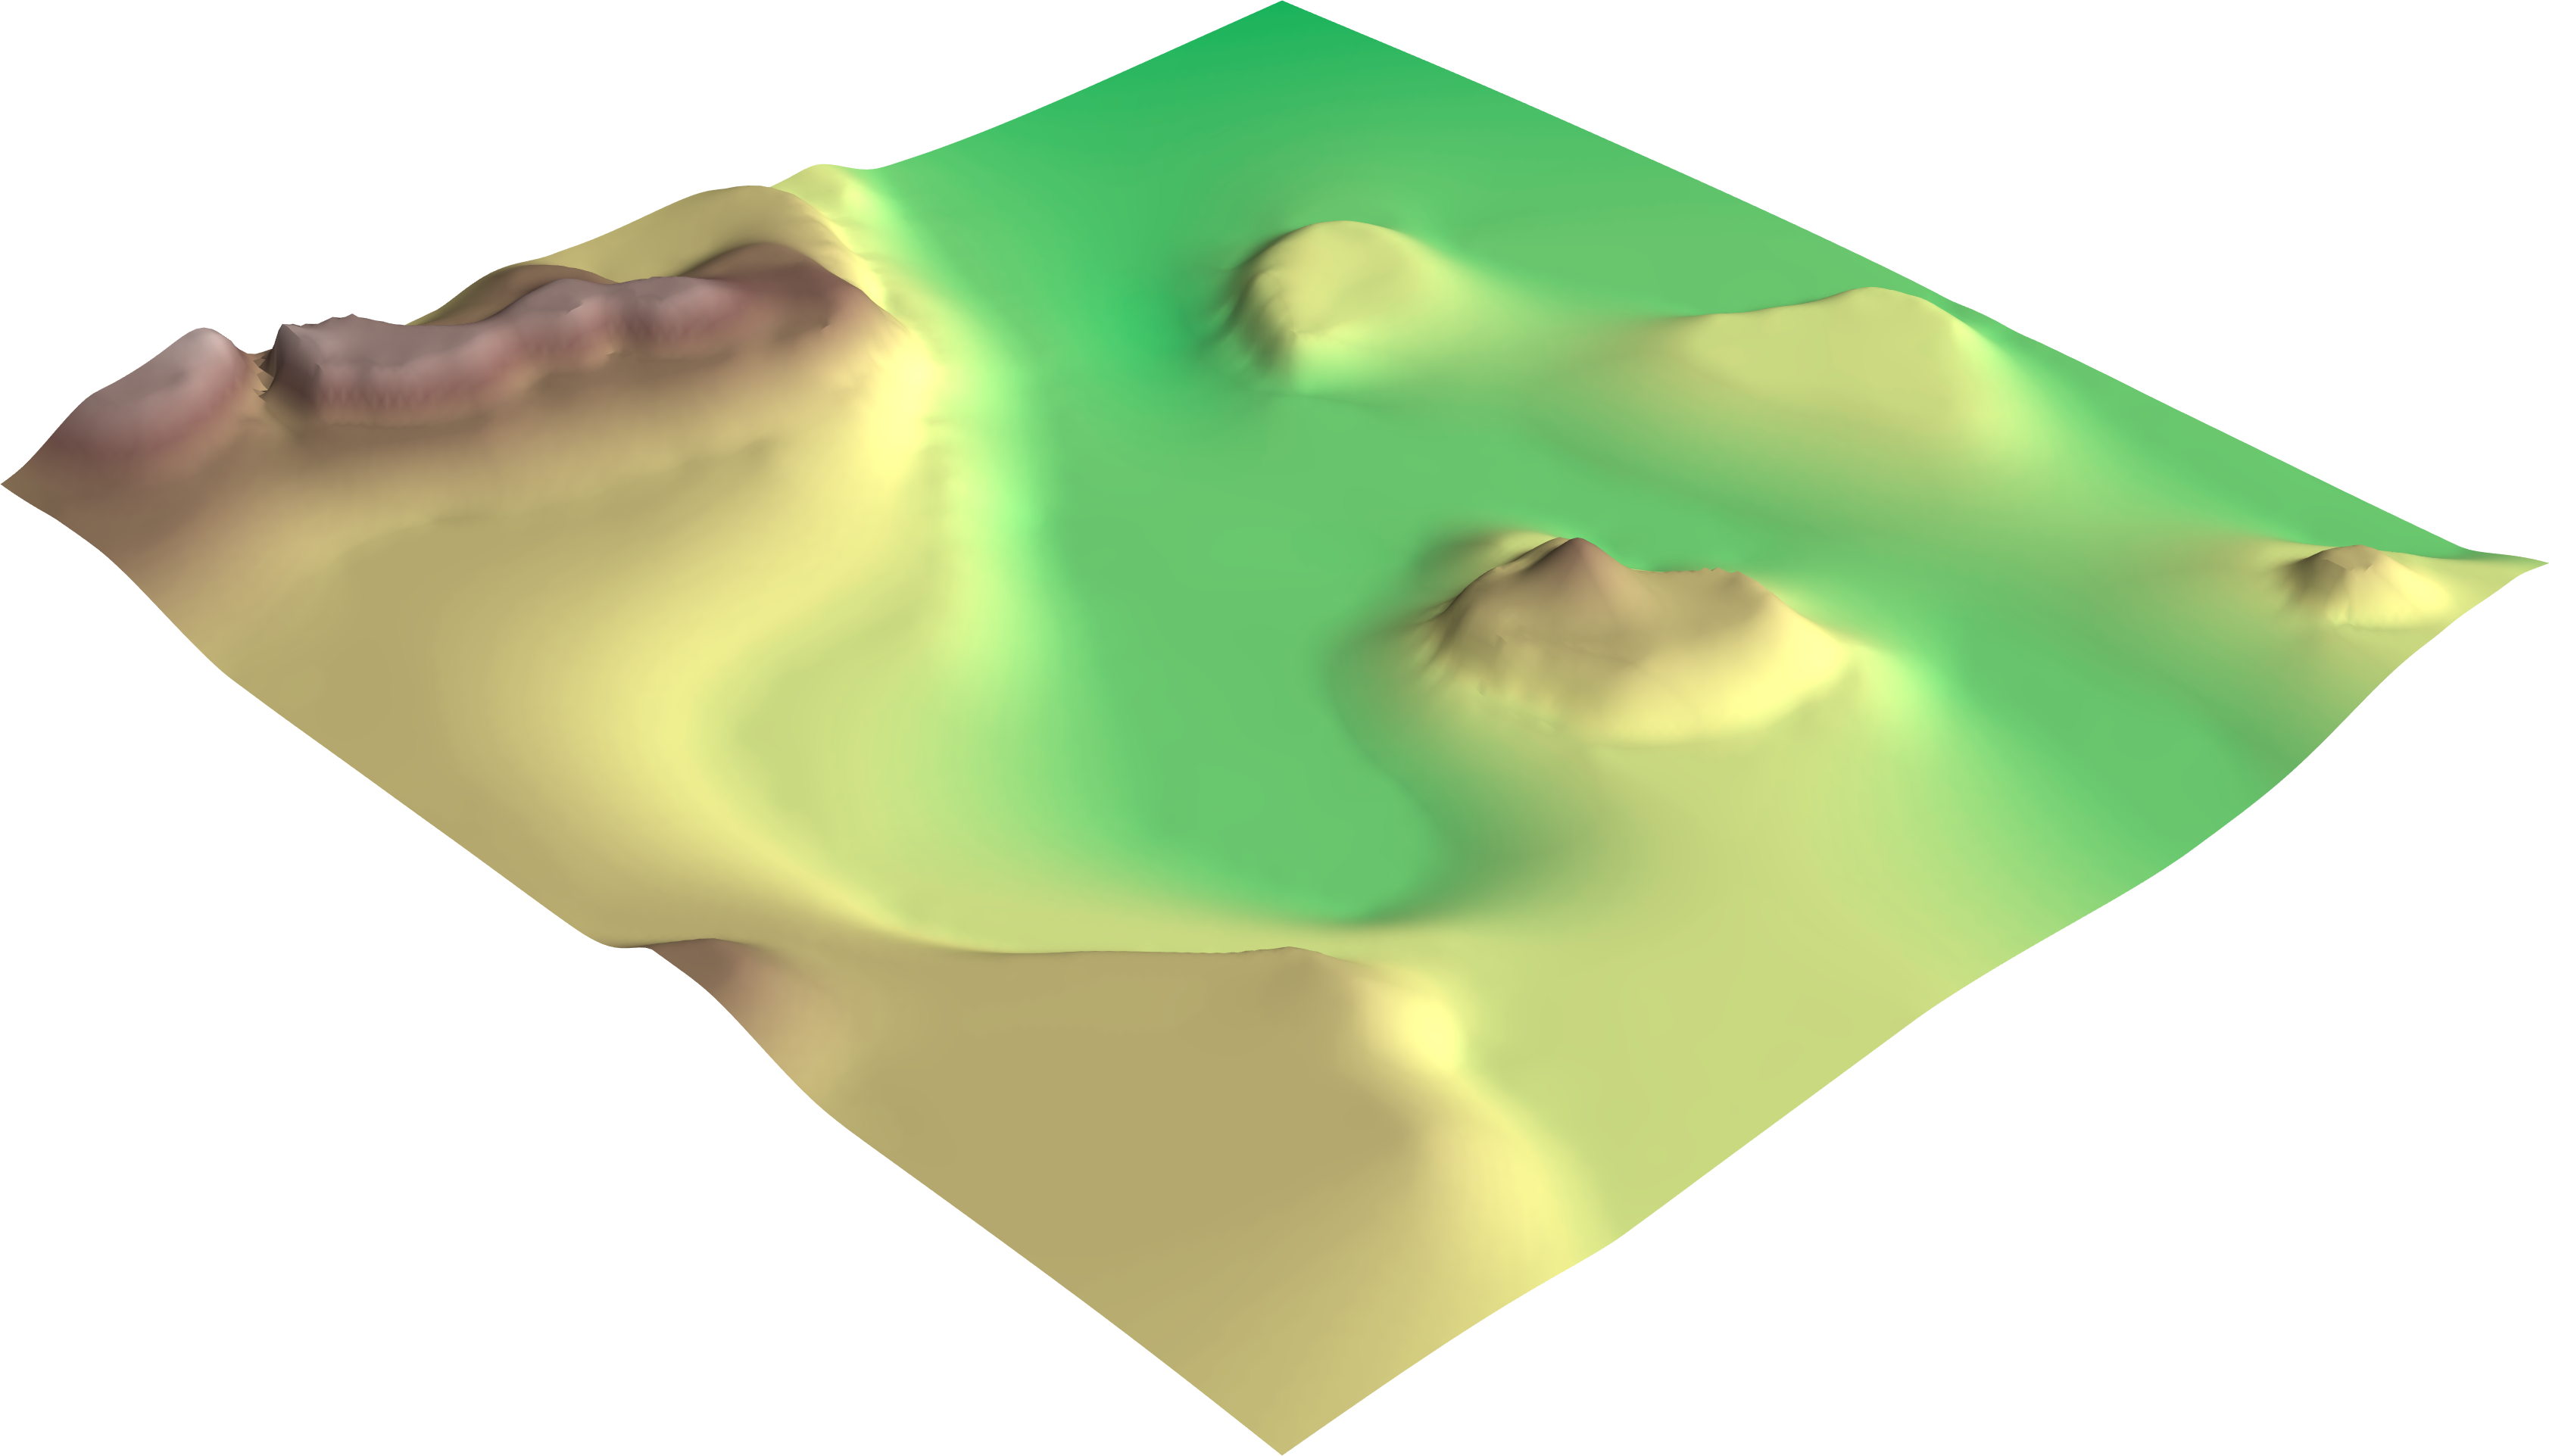
\includegraphics[width=\textwidth]{../images/differences/Radial_Basis_Thin_Plate_Spline_3D.png}
        % 2D_Contour_Interpolation.png: 1600x900 px, 100dpi, 40.64x22.86 cm, bb=0 0 1152 648
    \caption{Radial basis function interpolation using thin plate spline radial function.}
    \end{subfigure}
    \caption{Comparison of various interpolation methods using elevation data from UK ordnance tile NO44 (South of Forfar).}
    \label{fig:3D_discretized_comparison}
\end{figure}

In Figure \ref{fig:2D_discretized_comparison} and \ref{fig:3D_discretized_comparison} we compare these methods. We can immediately notice that neither of the methods is particularly accurate at the regions where no contour lines are available, in this case the NW corner of the tile. The methods using Delaunay tirangulation do not interpolate regions outside the convex hull of the isolated points at all, and radial basis function interpolation does produce reasonable estimates, but as can be seen on the right-most plot the absolute error in this region is still quite high.

Another issue with the Delaunay triangulation is that it doesn't produce smooth surfaces. This can be easily seen in Figure \ref{fig:3D_discretized_comparison} (a) and (b), where the triangles still remain visible when visualizing the surface. The Clough-Tocher scheme also introduces artifacts in forms of stretched valleys.

% \begin{figure}[H]
%     \centering
%     \begin{subfigure}{\textwidth}
%         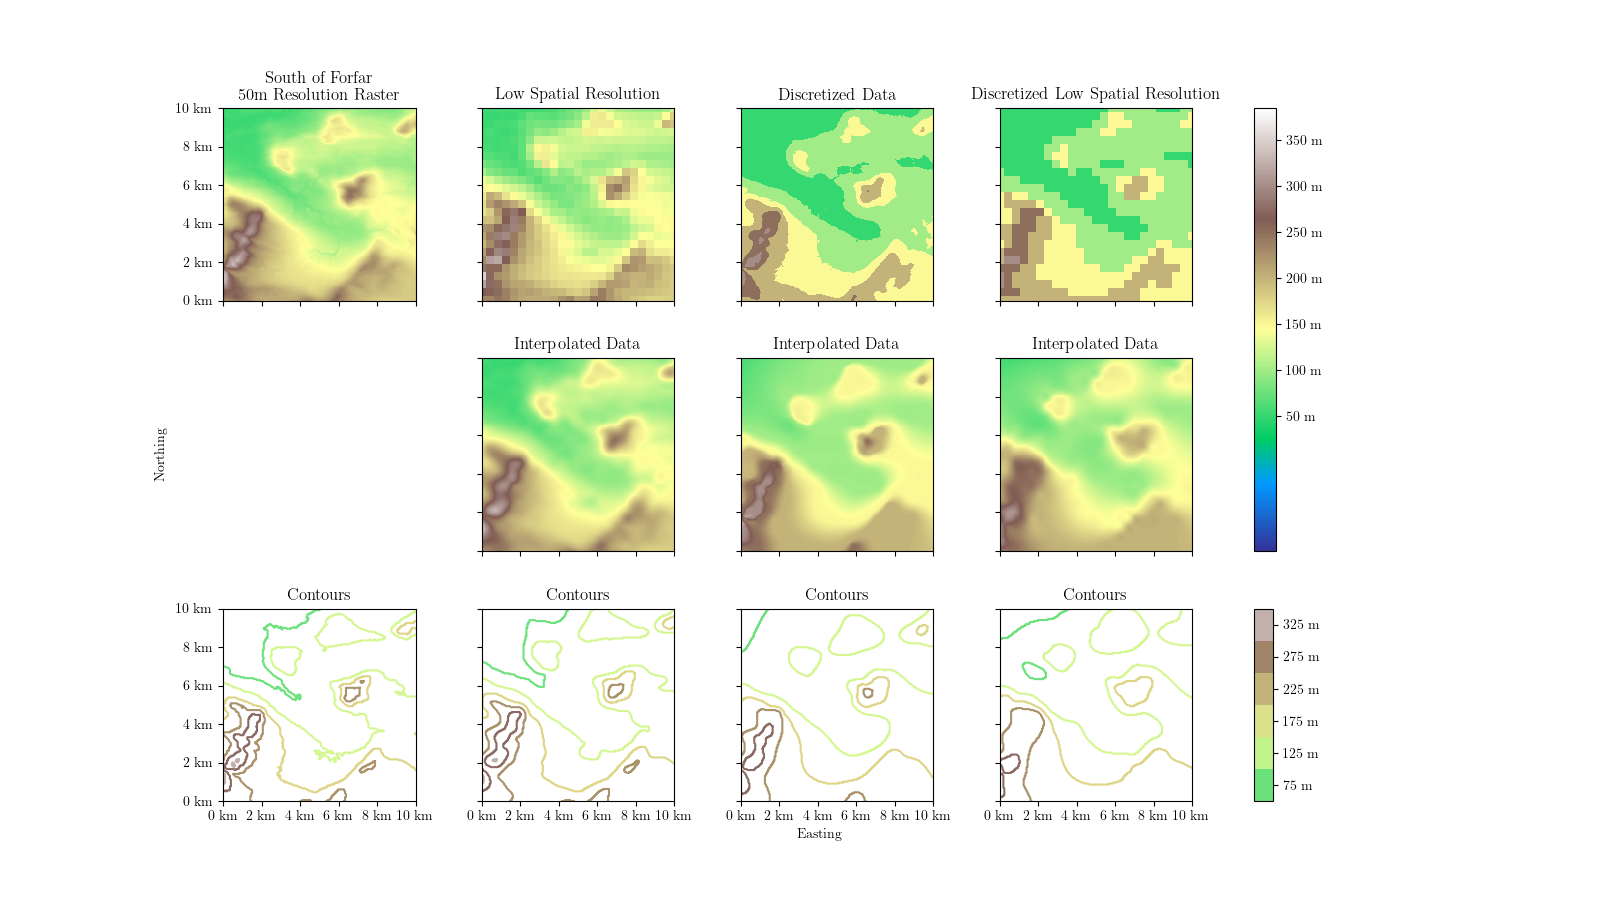
\includegraphics[width=1\textwidth]{../images/NO44/2D_Data_Interpolation.png}
%         % 2D_Contour_Interpolation.png: 1600x900 px, 100dpi, 40.64x22.86 cm, bb=0 0 1152 648
%     \caption{Elevation data from near Forfar (UK ordnance tile NO44)}
%     \end{subfigure}
%     \begin{subfigure}{\textwidth}
%         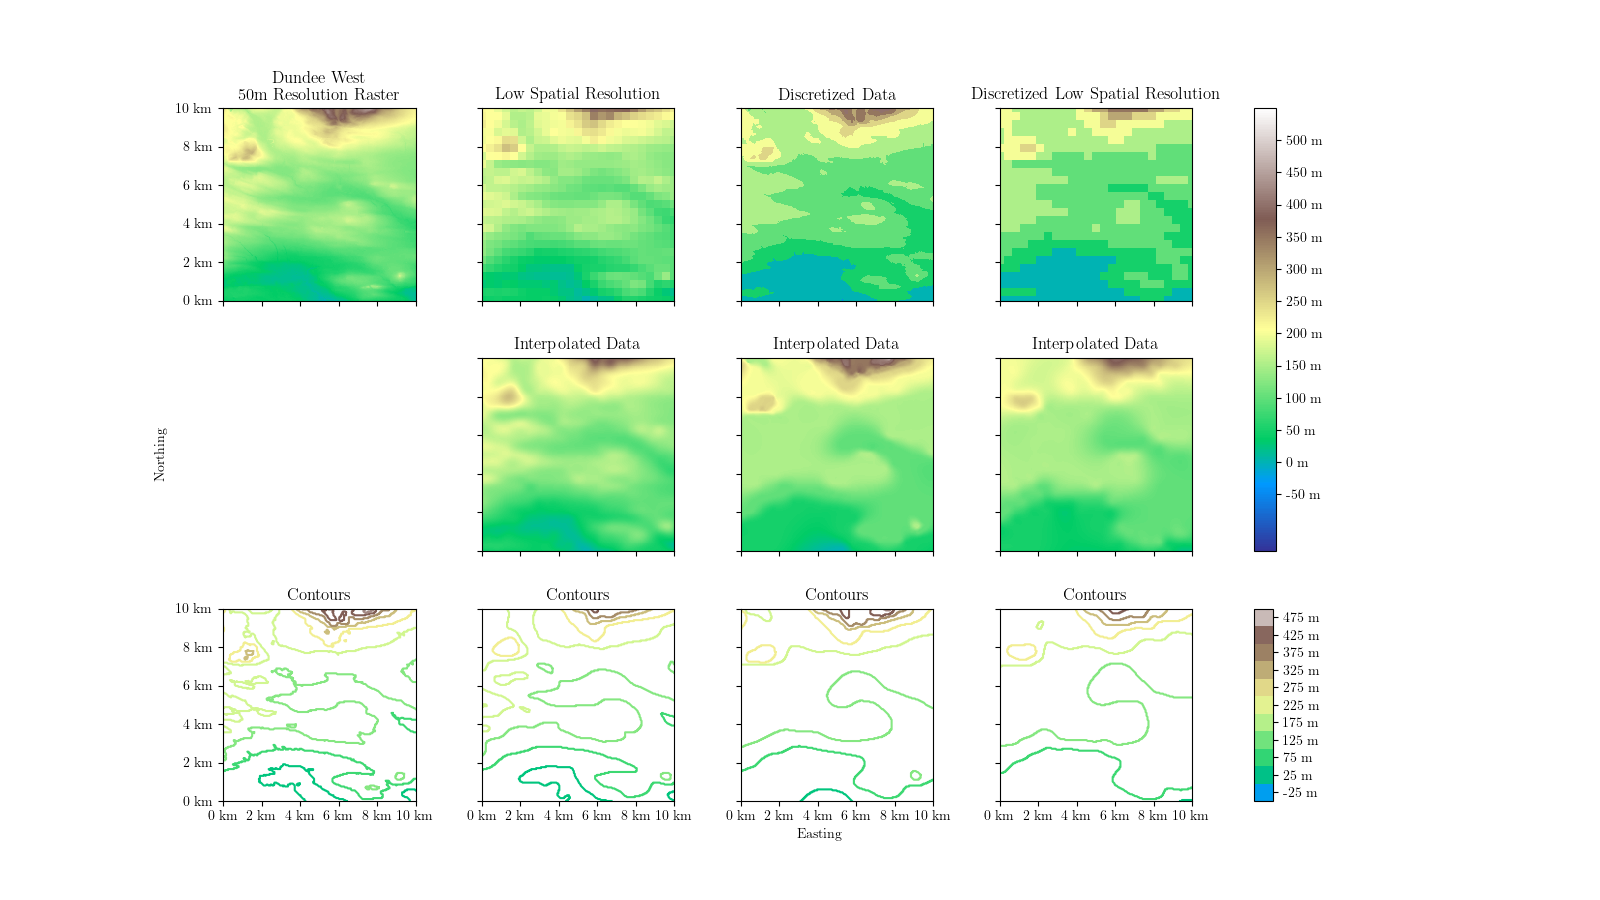
\includegraphics[width=1\textwidth]{../images/NO33/2D_Data_Interpolation.png}
%         % 2D_Contour_Interpolation.png: 1600x900 px, 100dpi, 40.64x22.86 cm, bb=0 0 1152 648
%     \caption{Elevation data from west Dundee (UK ordnance tile NO33)}
%     \end{subfigure}
%     \caption{Interpolation of elevation data with various resolution.}
%     \label{fig:2D_data}
% \end{figure}

\end{document}
